\begin{question}{22}{
    Een van de oefeningen van de Commando Elementaire Opleiding is een individuele verplaatsing in het donker langs verschillende checkpoints met enkel een kaart en kompas.
    Hierbij registreert de instructeur voor iedere cursist de totale tijd (afgerond op minuten) vanaf de start van de verplaatsing tot het bereiken van het eindpunt.

    Van de $19$ cursisten in de huidige lichting zijn de volgende verplaatsingstijden bijgehouden:
    \[
        150,\; 145,\; 120,\; 135,\; 122,\; 155,\; 165,\; 125,\; 142,\; 160,\; 138,\; 105,\; 140,\; 110,\; 200,\; 128,\; 130,\; 100,\; 115.
    \]
}
        \subquestion{11}{
            Teken een boxplot van de verplaatsingstijden.
            Schrijf hierbij de stappen op die je hebt uitgevoerd om de vijf getallen voor de boxplot te kunnen bepalen.
        }
        \answer{
            Om de vijf getallen voor de boxplot te bepalen, volgen we de volgende stappen:
            \begin{itemize}
                \item Sorteer de gegevens van laag naar hoog:
                
                {\scriptsize
                    $100,\; 105,\; 110,\; 115,\; 120,\; 122,\; 125,\; 128,\; 130,\; 135,\; 138,\; 140,\; 142,\; 145,\; 150,\; 155,\; 160,\; 165,\; 200$.\rubric{2}
                }
                \item De minimumwaarde is $100$ en de maximumwaarde is $200$.\rubric{1}
                \item Aangezien het aantal waarden $n = 19$, dus $n$ is oneven, is de mediaan (tweede kwartiel) de middelste (tiende) waarde: $135$.\rubric{1}
                \item Het eerste kwartiel $Q_1$ is de mediaan van de laagste \SI{50}{\percent} waarden (inclusief mediaan!) ($100$, $105$, $110$, $115$, $120$, $122$, $125$, $128$, $130$, $135$).
                Aangezien er $10$ waarden zijn, is het eerste kwartiel het gemiddelde van de vijfde en zesde waarde: $Q_1=\frac{120 + 122}{2} = 121$.\rubric{2}
                \item Het derde kwartiel $Q_3$ is de mediaan van de laagste \SI{50}{\percent} waarden (inclusief mediaan!) ($135$, $138$, $140$, $142$, $145$, $150$, $155$, $160$, $165$, $200$).
                Aangezien er $10$ waarden zijn, is het derde kwartiel het gemiddelde van de vijfde en zesde waarde: $Q_3=\frac{145+150}{2} = 147.5$.\rubric{1}
            \end{itemize}
            De vijf getallen voor de boxplot zijn dus:
            \[
                \text{Minimum} = 18, \quad Q_1 = 121, \quad \text{Mediaan} = 135, \quad Q_3 = 147.5, \quad \text{Maximum} = 200. 
            \]
            
            We tekenen de boxplot met \enquote{whiskers} van $Q_1 - 1.5 \times \IQR$ tot $Q_3 + 1.5 \times \IQR$, waarbij $\IQR = Q_3 - Q_1 = 147.5 - 121 = 26.5$. \rubric{1}
            De \enquote{whiskers} lopen van de kleinste niet-outlier boven $121 - 1.5 \times 26.5 = 81.25$ (oftewel $100$) tot de hoogste niet-outlier onder $147.5 + 1.5 \times 26.5 = 187.25$ (oftewel $165$).
            Er is één outlier, namelijk $200$. \rubric{1}
            \begin{center}
                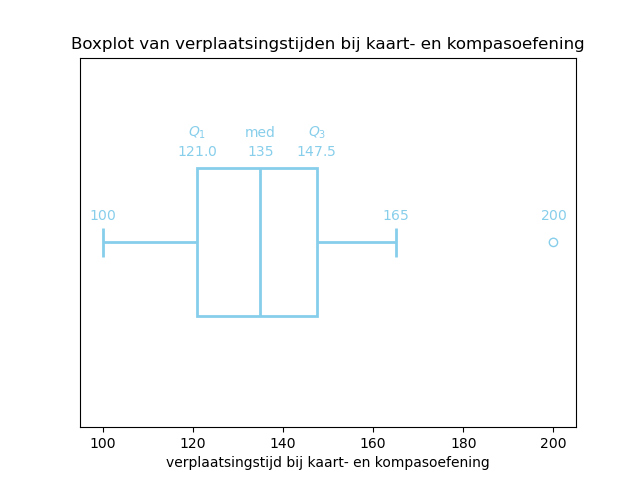
\includegraphics[width=\textwidth]{./20261016_exam_boxplot.png} \rubric{2}
            \end{center}

        }

        \subquestion{4}{
            Leg met behulp van de boxplot uit of het gemiddelde groter dan / kleiner dan / gelijk aan de mediaan is.
        }
        \answer{
            De boxplot is bijna symmetrisch te noemen in de mediaan.\rubric{1}
            Merk echter wel op dat er een extreem hoge waarde is van $200$, de enige outlier in deze boxplot\rubric{1}
            Deze outlier trekt het gemiddelde in verhouding omhoog, terwijl deze niet of nauwelijks invloed heeft op de mediaan.\rubric{1}
            Daarom kunnen we concluderen dat het gemiddelde van de reactietijden hoger ligt dan de mediaan van $22.5$ seconden. \rubric{1}

            (Maximaal 2 punten indien het gemiddelde direct wordt uitgerekend en geen connectie met de boxplot wordt gelegd.)
        }
        \subquestion{2}{
            % Noem één reden waarom deze steekproef mogelijk niet representatief is voor de reactietijden van alle militairen op de Trip van Zoudtlandtkazerne.
        }
        \answer{
            % Een mogelijke reden waarom deze steekproef niet representatief is, is dat de reactietijden alleen zijn gemeten van één specifiek peloton.\rubric{1}
            % De reactietijden kunnen variëren tussen verschillende pelotons vanwege verschillen in training, ervaring of andere factoren.
            % Hierdoor zou de resultaten van deze steekproef mogelijk niet generaliseerbaar kunnen zijn naar alle militairen in de Trip van Zoudtlandtkazerne. \rubric{1}
        }

        \subquestion{5}{
            % Tijdens de analyse ontdekt men dat er een fout is gemaakt bij het invoeren van de reactietijd van één van de militairen, en dat deze reactietijd eigenlijk $40$ seconden zou moeten zijn in plaats van $30$ seconden. 
            % Geef aan wat er zou veranderen aan de boxplot als deze fout wordt gecorrigeerd.
        }
        \answer{
            % Als de fout wordt gecorrigeerd en de reactietijd van $30$ seconden wordt vervangen door $40$ seconden, zal dit de maximumwaarde in de dataset veranderen van $35$ naar $40$.\rubric{1}
            % De minimumwaarde, het eerste kwartiel, de mediaan en het derde kwartiel zullen echter niet veranderen, omdat deze waarden niet worden beïnvloed door de hoogste waarde in de dataset.\rubric{2}
            % De whisker aan de rechterkant van de boxplot zal nu lopen tot de hoogste niet-outlier onder $25.5 + 1.5 \times 5.5 = 33.75$, oftewel $28$, en er zullen nu twee outliers zijn: $35$ en $40$. \rubric{2}
            % \begin{center}
            %     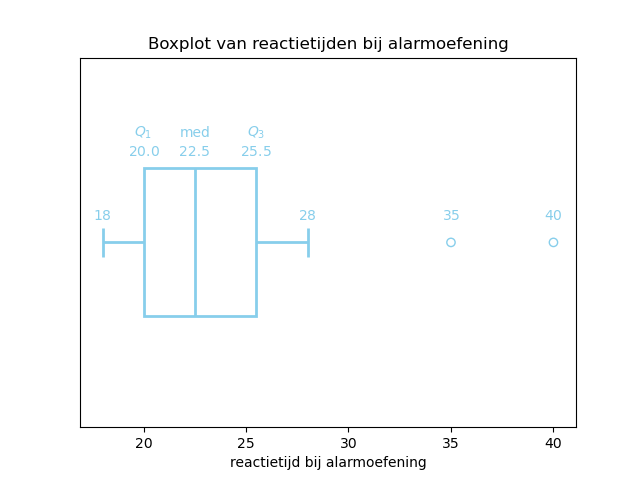
\includegraphics[width=\textwidth]{./20260605_exam_boxplot2.png}
            % \end{center}
        }
\end{question}